% Generated by ArticleSignalDiagrams. Opaque vector fills only.
\documentclass[10pt,tikz,border=5pt]{standalone}
\usepackage{lmodern}
\usetikzlibrary{fit}
\begin{document}
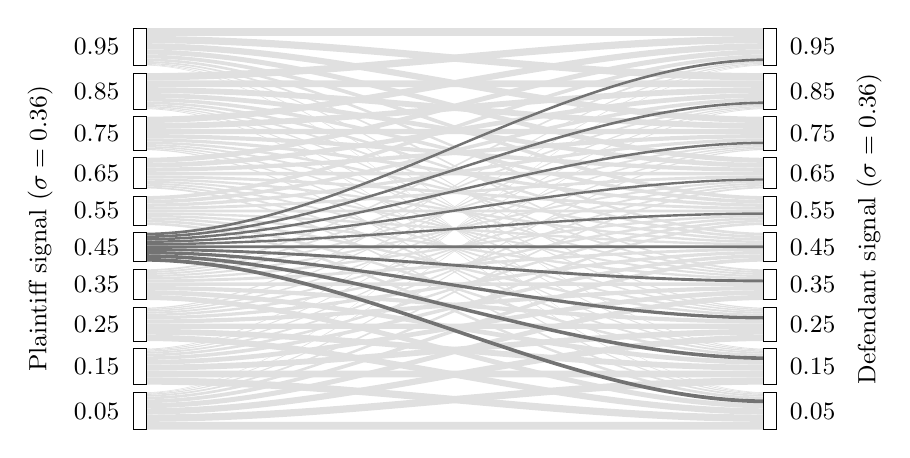
\begin{tikzpicture}[x=1cm,y=1cm,font=\small]\path[fill=black!12,draw=none] (3.3,-5.1) .. controls (6,-5.1) and (8.6,-5.1) .. (11.3,-5.1) -- (11.3,-5.000758) .. controls (8.6,-5.000758) and (6,-5.000758) .. (3.3,-5.000758) -- cycle;
\path[fill=black!12,draw=none] (3.3,-5.000758) .. controls (6,-5.000758) and (8.6,-4.527875) .. (11.3,-4.527875) -- (11.3,-4.435644) .. controls (8.6,-4.435644) and (6,-4.908528) .. (3.3,-4.908528) -- cycle;
\path[fill=black!12,draw=none] (3.3,-4.908528) .. controls (6,-4.908528) and (8.6,-3.973346) .. (11.3,-3.973346) -- (11.3,-3.893676) .. controls (8.6,-3.893676) and (6,-4.828858) .. (3.3,-4.828858) -- cycle;
\path[fill=black!12,draw=none] (3.3,-4.828858) .. controls (6,-4.828858) and (8.6,-3.45213) .. (11.3,-3.45213) -- (11.3,-3.388061) .. controls (8.6,-3.388061) and (6,-4.764788) .. (3.3,-4.764788) -- cycle;
\path[fill=black!12,draw=none] (3.3,-4.764788) .. controls (6,-4.764788) and (8.6,-2.965329) .. (11.3,-2.965329) -- (11.3,-2.917198) .. controls (8.6,-2.917198) and (6,-4.716658) .. (3.3,-4.716658) -- cycle;
\path[fill=black!12,draw=none] (3.3,-4.716658) .. controls (6,-4.716658) and (8.6,-2.5) .. (11.3,-2.5) -- (11.3,-2.465996) .. controls (8.6,-2.465996) and (6,-4.682655) .. (3.3,-4.682655) -- cycle;
\path[fill=black!12,draw=none] (3.3,-4.682655) .. controls (6,-4.682655) and (8.6,-2.034671) .. (11.3,-2.034671) -- (11.3,-2.01178) .. controls (8.6,-2.01178) and (6,-4.659763) .. (3.3,-4.659763) -- cycle;
\path[fill=black!12,draw=none] (3.3,-4.659763) .. controls (6,-4.659763) and (8.6,-1.54787) .. (11.3,-1.54787) -- (11.3,-1.532841) .. controls (8.6,-1.532841) and (6,-4.644734) .. (3.3,-4.644734) -- cycle;
\path[fill=black!12,draw=none] (3.3,-4.644734) .. controls (6,-4.644734) and (8.6,-1.026654) .. (11.3,-1.026654) -- (11.3,-1.016697) .. controls (8.6,-1.016697) and (6,-4.634777) .. (3.3,-4.634777) -- cycle;
\path[fill=black!12,draw=none] (3.3,-4.634777) .. controls (6,-4.634777) and (8.6,-0.472125) .. (11.3,-0.472125) -- (11.3,-0.465223) .. controls (8.6,-0.465223) and (6,-4.627875) .. (3.3,-4.627875) -- cycle;
\path[fill=black!12,draw=none] (3.3,-4.527875) .. controls (6,-4.527875) and (8.6,-5.000758) .. (11.3,-5.000758) -- (11.3,-4.908528) .. controls (8.6,-4.908528) and (6,-4.435644) .. (3.3,-4.435644) -- cycle;
\path[fill=black!12,draw=none] (3.3,-4.435644) .. controls (6,-4.435644) and (8.6,-4.435644) .. (11.3,-4.435644) -- (11.3,-4.349803) .. controls (8.6,-4.349803) and (6,-4.349803) .. (3.3,-4.349803) -- cycle;
\path[fill=black!12,draw=none] (3.3,-4.349803) .. controls (6,-4.349803) and (8.6,-3.893676) .. (11.3,-3.893676) -- (11.3,-3.819295) .. controls (8.6,-3.819295) and (6,-4.275422) .. (3.3,-4.275422) -- cycle;
\path[fill=black!12,draw=none] (3.3,-4.275422) .. controls (6,-4.275422) and (8.6,-3.388061) .. (11.3,-3.388061) -- (11.3,-3.327856) .. controls (8.6,-3.327856) and (6,-4.215217) .. (3.3,-4.215217) -- cycle;
\path[fill=black!12,draw=none] (3.3,-4.215217) .. controls (6,-4.215217) and (8.6,-2.917198) .. (11.3,-2.917198) -- (11.3,-2.871369) .. controls (8.6,-2.871369) and (6,-4.169388) .. (3.3,-4.169388) -- cycle;
\path[fill=black!12,draw=none] (3.3,-4.169388) .. controls (6,-4.169388) and (8.6,-2.465996) .. (11.3,-2.465996) -- (11.3,-2.432753) .. controls (8.6,-2.432753) and (6,-4.136144) .. (3.3,-4.136144) -- cycle;
\path[fill=black!12,draw=none] (3.3,-4.136144) .. controls (6,-4.136144) and (8.6,-2.01178) .. (11.3,-2.01178) -- (11.3,-1.988264) .. controls (8.6,-1.988264) and (6,-4.112629) .. (3.3,-4.112629) -- cycle;
\path[fill=black!12,draw=none] (3.3,-4.112629) .. controls (6,-4.112629) and (8.6,-1.532841) .. (11.3,-1.532841) -- (11.3,-1.516053) .. controls (8.6,-1.516053) and (6,-4.095841) .. (3.3,-4.095841) -- cycle;
\path[fill=black!12,draw=none] (3.3,-4.095841) .. controls (6,-4.095841) and (8.6,-1.016697) .. (11.3,-1.016697) -- (11.3,-1.004159) .. controls (8.6,-1.004159) and (6,-4.083303) .. (3.3,-4.083303) -- cycle;
\path[fill=black!12,draw=none] (3.3,-4.083303) .. controls (6,-4.083303) and (8.6,-0.465223) .. (11.3,-0.465223) -- (11.3,-0.455266) .. controls (8.6,-0.455266) and (6,-4.073346) .. (3.3,-4.073346) -- cycle;
\path[fill=black!12,draw=none] (3.3,-3.973346) .. controls (6,-3.973346) and (8.6,-4.908528) .. (11.3,-4.908528) -- (11.3,-4.828858) .. controls (8.6,-4.828858) and (6,-3.893676) .. (3.3,-3.893676) -- cycle;
\path[fill=black!12,draw=none] (3.3,-3.893676) .. controls (6,-3.893676) and (8.6,-4.349803) .. (11.3,-4.349803) -- (11.3,-4.275422) .. controls (8.6,-4.275422) and (6,-3.819295) .. (3.3,-3.819295) -- cycle;
\path[fill=black!12,draw=none] (3.3,-3.819295) .. controls (6,-3.819295) and (8.6,-3.819295) .. (11.3,-3.819295) -- (11.3,-3.754426) .. controls (8.6,-3.754426) and (6,-3.754426) .. (3.3,-3.754426) -- cycle;
\path[fill=black!12,draw=none] (3.3,-3.754426) .. controls (6,-3.754426) and (8.6,-3.327856) .. (11.3,-3.327856) -- (11.3,-3.274651) .. controls (8.6,-3.274651) and (6,-3.701221) .. (3.3,-3.701221) -- cycle;
\path[fill=black!12,draw=none] (3.3,-3.701221) .. controls (6,-3.701221) and (8.6,-2.871369) .. (11.3,-2.871369) -- (11.3,-2.829786) .. controls (8.6,-2.829786) and (6,-3.659638) .. (3.3,-3.659638) -- cycle;
\path[fill=black!12,draw=none] (3.3,-3.659638) .. controls (6,-3.659638) and (8.6,-2.432753) .. (11.3,-2.432753) -- (11.3,-2.401059) .. controls (8.6,-2.401059) and (6,-3.627944) .. (3.3,-3.627944) -- cycle;
\path[fill=black!12,draw=none] (3.3,-3.627944) .. controls (6,-3.627944) and (8.6,-1.988264) .. (11.3,-1.988264) -- (11.3,-1.963885) .. controls (8.6,-1.963885) and (6,-3.603565) .. (3.3,-3.603565) -- cycle;
\path[fill=black!12,draw=none] (3.3,-3.603565) .. controls (6,-3.603565) and (8.6,-1.516053) .. (11.3,-1.516053) -- (11.3,-1.496435) .. controls (8.6,-1.496435) and (6,-3.583947) .. (3.3,-3.583947) -- cycle;
\path[fill=black!12,draw=none] (3.3,-3.583947) .. controls (6,-3.583947) and (8.6,-1.004159) .. (11.3,-1.004159) -- (11.3,-0.987371) .. controls (8.6,-0.987371) and (6,-3.567159) .. (3.3,-3.567159) -- cycle;
\path[fill=black!12,draw=none] (3.3,-3.567159) .. controls (6,-3.567159) and (8.6,-0.455266) .. (11.3,-0.455266) -- (11.3,-0.440237) .. controls (8.6,-0.440237) and (6,-3.55213) .. (3.3,-3.55213) -- cycle;
\path[fill=black!12,draw=none] (3.3,-3.45213) .. controls (6,-3.45213) and (8.6,-4.828858) .. (11.3,-4.828858) -- (11.3,-4.764788) .. controls (8.6,-4.764788) and (6,-3.388061) .. (3.3,-3.388061) -- cycle;
\path[fill=black!12,draw=none] (3.3,-3.388061) .. controls (6,-3.388061) and (8.6,-4.275422) .. (11.3,-4.275422) -- (11.3,-4.215217) .. controls (8.6,-4.215217) and (6,-3.327856) .. (3.3,-3.327856) -- cycle;
\path[fill=black!12,draw=none] (3.3,-3.327856) .. controls (6,-3.327856) and (8.6,-3.754426) .. (11.3,-3.754426) -- (11.3,-3.701221) .. controls (8.6,-3.701221) and (6,-3.274651) .. (3.3,-3.274651) -- cycle;
\path[fill=black!12,draw=none] (3.3,-3.274651) .. controls (6,-3.274651) and (8.6,-3.274651) .. (11.3,-3.274651) -- (11.3,-3.229847) .. controls (8.6,-3.229847) and (6,-3.229847) .. (3.3,-3.229847) -- cycle;
\path[fill=black!12,draw=none] (3.3,-3.229847) .. controls (6,-3.229847) and (8.6,-2.829786) .. (11.3,-2.829786) -- (11.3,-2.792991) .. controls (8.6,-2.792991) and (6,-3.193052) .. (3.3,-3.193052) -- cycle;
\path[fill=black!12,draw=none] (3.3,-3.193052) .. controls (6,-3.193052) and (8.6,-2.401059) .. (11.3,-2.401059) -- (11.3,-2.370564) .. controls (8.6,-2.370564) and (6,-3.162556) .. (3.3,-3.162556) -- cycle;
\path[fill=black!12,draw=none] (3.3,-3.162556) .. controls (6,-3.162556) and (8.6,-1.963885) .. (11.3,-1.963885) -- (11.3,-1.937444) .. controls (8.6,-1.937444) and (6,-3.136115) .. (3.3,-3.136115) -- cycle;
\path[fill=black!12,draw=none] (3.3,-3.136115) .. controls (6,-3.136115) and (8.6,-1.496435) .. (11.3,-1.496435) -- (11.3,-1.472056) .. controls (8.6,-1.472056) and (6,-3.111736) .. (3.3,-3.111736) -- cycle;
\path[fill=black!12,draw=none] (3.3,-3.111736) .. controls (6,-3.111736) and (8.6,-0.987371) .. (11.3,-0.987371) -- (11.3,-0.963856) .. controls (8.6,-0.963856) and (6,-3.08822) .. (3.3,-3.08822) -- cycle;
\path[fill=black!12,draw=none] (3.3,-3.08822) .. controls (6,-3.08822) and (8.6,-0.440237) .. (11.3,-0.440237) -- (11.3,-0.417345) .. controls (8.6,-0.417345) and (6,-3.065329) .. (3.3,-3.065329) -- cycle;
\path[fill=black!12,draw=none] (3.3,-2.5) .. controls (6,-2.5) and (8.6,-4.716658) .. (11.3,-4.716658) -- (11.3,-4.682655) .. controls (8.6,-4.682655) and (6,-2.465996) .. (3.3,-2.465996) -- cycle;
\path[fill=black!12,draw=none] (3.3,-2.465996) .. controls (6,-2.465996) and (8.6,-4.169388) .. (11.3,-4.169388) -- (11.3,-4.136144) .. controls (8.6,-4.136144) and (6,-2.432753) .. (3.3,-2.432753) -- cycle;
\path[fill=black!12,draw=none] (3.3,-2.432753) .. controls (6,-2.432753) and (8.6,-3.659638) .. (11.3,-3.659638) -- (11.3,-3.627944) .. controls (8.6,-3.627944) and (6,-2.401059) .. (3.3,-2.401059) -- cycle;
\path[fill=black!12,draw=none] (3.3,-2.401059) .. controls (6,-2.401059) and (8.6,-3.193052) .. (11.3,-3.193052) -- (11.3,-3.162556) .. controls (8.6,-3.162556) and (6,-2.370564) .. (3.3,-2.370564) -- cycle;
\path[fill=black!12,draw=none] (3.3,-2.370564) .. controls (6,-2.370564) and (8.6,-2.760133) .. (11.3,-2.760133) -- (11.3,-2.729436) .. controls (8.6,-2.729436) and (6,-2.339867) .. (3.3,-2.339867) -- cycle;
\path[fill=black!12,draw=none] (3.3,-2.339867) .. controls (6,-2.339867) and (8.6,-2.339867) .. (11.3,-2.339867) -- (11.3,-2.307009) .. controls (8.6,-2.307009) and (6,-2.307009) .. (3.3,-2.307009) -- cycle;
\path[fill=black!12,draw=none] (3.3,-2.307009) .. controls (6,-2.307009) and (8.6,-1.906948) .. (11.3,-1.906948) -- (11.3,-1.870153) .. controls (8.6,-1.870153) and (6,-2.270214) .. (3.3,-2.270214) -- cycle;
\path[fill=black!12,draw=none] (3.3,-2.270214) .. controls (6,-2.270214) and (8.6,-1.440362) .. (11.3,-1.440362) -- (11.3,-1.398779) .. controls (8.6,-1.398779) and (6,-2.228631) .. (3.3,-2.228631) -- cycle;
\path[fill=black!12,draw=none] (3.3,-2.228631) .. controls (6,-2.228631) and (8.6,-0.930612) .. (11.3,-0.930612) -- (11.3,-0.884783) .. controls (8.6,-0.884783) and (6,-2.182802) .. (3.3,-2.182802) -- cycle;
\path[fill=black!12,draw=none] (3.3,-2.182802) .. controls (6,-2.182802) and (8.6,-0.383342) .. (11.3,-0.383342) -- (11.3,-0.335212) .. controls (8.6,-0.335212) and (6,-2.134671) .. (3.3,-2.134671) -- cycle;
\path[fill=black!12,draw=none] (3.3,-2.034671) .. controls (6,-2.034671) and (8.6,-4.682655) .. (11.3,-4.682655) -- (11.3,-4.659763) .. controls (8.6,-4.659763) and (6,-2.01178) .. (3.3,-2.01178) -- cycle;
\path[fill=black!12,draw=none] (3.3,-2.01178) .. controls (6,-2.01178) and (8.6,-4.136144) .. (11.3,-4.136144) -- (11.3,-4.112629) .. controls (8.6,-4.112629) and (6,-1.988264) .. (3.3,-1.988264) -- cycle;
\path[fill=black!12,draw=none] (3.3,-1.988264) .. controls (6,-1.988264) and (8.6,-3.627944) .. (11.3,-3.627944) -- (11.3,-3.603565) .. controls (8.6,-3.603565) and (6,-1.963885) .. (3.3,-1.963885) -- cycle;
\path[fill=black!12,draw=none] (3.3,-1.963885) .. controls (6,-1.963885) and (8.6,-3.162556) .. (11.3,-3.162556) -- (11.3,-3.136115) .. controls (8.6,-3.136115) and (6,-1.937444) .. (3.3,-1.937444) -- cycle;
\path[fill=black!12,draw=none] (3.3,-1.937444) .. controls (6,-1.937444) and (8.6,-2.729436) .. (11.3,-2.729436) -- (11.3,-2.698941) .. controls (8.6,-2.698941) and (6,-1.906948) .. (3.3,-1.906948) -- cycle;
\path[fill=black!12,draw=none] (3.3,-1.906948) .. controls (6,-1.906948) and (8.6,-2.307009) .. (11.3,-2.307009) -- (11.3,-2.270214) .. controls (8.6,-2.270214) and (6,-1.870153) .. (3.3,-1.870153) -- cycle;
\path[fill=black!12,draw=none] (3.3,-1.870153) .. controls (6,-1.870153) and (8.6,-1.870153) .. (11.3,-1.870153) -- (11.3,-1.825349) .. controls (8.6,-1.825349) and (6,-1.825349) .. (3.3,-1.825349) -- cycle;
\path[fill=black!12,draw=none] (3.3,-1.825349) .. controls (6,-1.825349) and (8.6,-1.398779) .. (11.3,-1.398779) -- (11.3,-1.345574) .. controls (8.6,-1.345574) and (6,-1.772144) .. (3.3,-1.772144) -- cycle;
\path[fill=black!12,draw=none] (3.3,-1.772144) .. controls (6,-1.772144) and (8.6,-0.884783) .. (11.3,-0.884783) -- (11.3,-0.824578) .. controls (8.6,-0.824578) and (6,-1.711939) .. (3.3,-1.711939) -- cycle;
\path[fill=black!12,draw=none] (3.3,-1.711939) .. controls (6,-1.711939) and (8.6,-0.335212) .. (11.3,-0.335212) -- (11.3,-0.271142) .. controls (8.6,-0.271142) and (6,-1.64787) .. (3.3,-1.64787) -- cycle;
\path[fill=black!12,draw=none] (3.3,-1.54787) .. controls (6,-1.54787) and (8.6,-4.659763) .. (11.3,-4.659763) -- (11.3,-4.644734) .. controls (8.6,-4.644734) and (6,-1.532841) .. (3.3,-1.532841) -- cycle;
\path[fill=black!12,draw=none] (3.3,-1.532841) .. controls (6,-1.532841) and (8.6,-4.112629) .. (11.3,-4.112629) -- (11.3,-4.095841) .. controls (8.6,-4.095841) and (6,-1.516053) .. (3.3,-1.516053) -- cycle;
\path[fill=black!12,draw=none] (3.3,-1.516053) .. controls (6,-1.516053) and (8.6,-3.603565) .. (11.3,-3.603565) -- (11.3,-3.583947) .. controls (8.6,-3.583947) and (6,-1.496435) .. (3.3,-1.496435) -- cycle;
\path[fill=black!12,draw=none] (3.3,-1.496435) .. controls (6,-1.496435) and (8.6,-3.136115) .. (11.3,-3.136115) -- (11.3,-3.111736) .. controls (8.6,-3.111736) and (6,-1.472056) .. (3.3,-1.472056) -- cycle;
\path[fill=black!12,draw=none] (3.3,-1.472056) .. controls (6,-1.472056) and (8.6,-2.698941) .. (11.3,-2.698941) -- (11.3,-2.667247) .. controls (8.6,-2.667247) and (6,-1.440362) .. (3.3,-1.440362) -- cycle;
\path[fill=black!12,draw=none] (3.3,-1.440362) .. controls (6,-1.440362) and (8.6,-2.270214) .. (11.3,-2.270214) -- (11.3,-2.228631) .. controls (8.6,-2.228631) and (6,-1.398779) .. (3.3,-1.398779) -- cycle;
\path[fill=black!12,draw=none] (3.3,-1.398779) .. controls (6,-1.398779) and (8.6,-1.825349) .. (11.3,-1.825349) -- (11.3,-1.772144) .. controls (8.6,-1.772144) and (6,-1.345574) .. (3.3,-1.345574) -- cycle;
\path[fill=black!12,draw=none] (3.3,-1.345574) .. controls (6,-1.345574) and (8.6,-1.345574) .. (11.3,-1.345574) -- (11.3,-1.280705) .. controls (8.6,-1.280705) and (6,-1.280705) .. (3.3,-1.280705) -- cycle;
\path[fill=black!12,draw=none] (3.3,-1.280705) .. controls (6,-1.280705) and (8.6,-0.824578) .. (11.3,-0.824578) -- (11.3,-0.750197) .. controls (8.6,-0.750197) and (6,-1.206324) .. (3.3,-1.206324) -- cycle;
\path[fill=black!12,draw=none] (3.3,-1.206324) .. controls (6,-1.206324) and (8.6,-0.271142) .. (11.3,-0.271142) -- (11.3,-0.191472) .. controls (8.6,-0.191472) and (6,-1.126654) .. (3.3,-1.126654) -- cycle;
\path[fill=black!12,draw=none] (3.3,-1.026654) .. controls (6,-1.026654) and (8.6,-4.644734) .. (11.3,-4.644734) -- (11.3,-4.634777) .. controls (8.6,-4.634777) and (6,-1.016697) .. (3.3,-1.016697) -- cycle;
\path[fill=black!12,draw=none] (3.3,-1.016697) .. controls (6,-1.016697) and (8.6,-4.095841) .. (11.3,-4.095841) -- (11.3,-4.083303) .. controls (8.6,-4.083303) and (6,-1.004159) .. (3.3,-1.004159) -- cycle;
\path[fill=black!12,draw=none] (3.3,-1.004159) .. controls (6,-1.004159) and (8.6,-3.583947) .. (11.3,-3.583947) -- (11.3,-3.567159) .. controls (8.6,-3.567159) and (6,-0.987371) .. (3.3,-0.987371) -- cycle;
\path[fill=black!12,draw=none] (3.3,-0.987371) .. controls (6,-0.987371) and (8.6,-3.111736) .. (11.3,-3.111736) -- (11.3,-3.08822) .. controls (8.6,-3.08822) and (6,-0.963856) .. (3.3,-0.963856) -- cycle;
\path[fill=black!12,draw=none] (3.3,-0.963856) .. controls (6,-0.963856) and (8.6,-2.667247) .. (11.3,-2.667247) -- (11.3,-2.634004) .. controls (8.6,-2.634004) and (6,-0.930612) .. (3.3,-0.930612) -- cycle;
\path[fill=black!12,draw=none] (3.3,-0.930612) .. controls (6,-0.930612) and (8.6,-2.228631) .. (11.3,-2.228631) -- (11.3,-2.182802) .. controls (8.6,-2.182802) and (6,-0.884783) .. (3.3,-0.884783) -- cycle;
\path[fill=black!12,draw=none] (3.3,-0.884783) .. controls (6,-0.884783) and (8.6,-1.772144) .. (11.3,-1.772144) -- (11.3,-1.711939) .. controls (8.6,-1.711939) and (6,-0.824578) .. (3.3,-0.824578) -- cycle;
\path[fill=black!12,draw=none] (3.3,-0.824578) .. controls (6,-0.824578) and (8.6,-1.280705) .. (11.3,-1.280705) -- (11.3,-1.206324) .. controls (8.6,-1.206324) and (6,-0.750197) .. (3.3,-0.750197) -- cycle;
\path[fill=black!12,draw=none] (3.3,-0.750197) .. controls (6,-0.750197) and (8.6,-0.750197) .. (11.3,-0.750197) -- (11.3,-0.664356) .. controls (8.6,-0.664356) and (6,-0.664356) .. (3.3,-0.664356) -- cycle;
\path[fill=black!12,draw=none] (3.3,-0.664356) .. controls (6,-0.664356) and (8.6,-0.191472) .. (11.3,-0.191472) -- (11.3,-0.099242) .. controls (8.6,-0.099242) and (6,-0.572125) .. (3.3,-0.572125) -- cycle;
\path[fill=black!12,draw=none] (3.3,-0.472125) .. controls (6,-0.472125) and (8.6,-4.634777) .. (11.3,-4.634777) -- (11.3,-4.627875) .. controls (8.6,-4.627875) and (6,-0.465223) .. (3.3,-0.465223) -- cycle;
\path[fill=black!12,draw=none] (3.3,-0.465223) .. controls (6,-0.465223) and (8.6,-4.083303) .. (11.3,-4.083303) -- (11.3,-4.073346) .. controls (8.6,-4.073346) and (6,-0.455266) .. (3.3,-0.455266) -- cycle;
\path[fill=black!12,draw=none] (3.3,-0.455266) .. controls (6,-0.455266) and (8.6,-3.567159) .. (11.3,-3.567159) -- (11.3,-3.55213) .. controls (8.6,-3.55213) and (6,-0.440237) .. (3.3,-0.440237) -- cycle;
\path[fill=black!12,draw=none] (3.3,-0.440237) .. controls (6,-0.440237) and (8.6,-3.08822) .. (11.3,-3.08822) -- (11.3,-3.065329) .. controls (8.6,-3.065329) and (6,-0.417345) .. (3.3,-0.417345) -- cycle;
\path[fill=black!12,draw=none] (3.3,-0.417345) .. controls (6,-0.417345) and (8.6,-2.634004) .. (11.3,-2.634004) -- (11.3,-2.6) .. controls (8.6,-2.6) and (6,-0.383342) .. (3.3,-0.383342) -- cycle;
\path[fill=black!12,draw=none] (3.3,-0.383342) .. controls (6,-0.383342) and (8.6,-2.182802) .. (11.3,-2.182802) -- (11.3,-2.134671) .. controls (8.6,-2.134671) and (6,-0.335212) .. (3.3,-0.335212) -- cycle;
\path[fill=black!12,draw=none] (3.3,-0.335212) .. controls (6,-0.335212) and (8.6,-1.711939) .. (11.3,-1.711939) -- (11.3,-1.64787) .. controls (8.6,-1.64787) and (6,-0.271142) .. (3.3,-0.271142) -- cycle;
\path[fill=black!12,draw=none] (3.3,-0.271142) .. controls (6,-0.271142) and (8.6,-1.206324) .. (11.3,-1.206324) -- (11.3,-1.126654) .. controls (8.6,-1.126654) and (6,-0.191472) .. (3.3,-0.191472) -- cycle;
\path[fill=black!12,draw=none] (3.3,-0.191472) .. controls (6,-0.191472) and (8.6,-0.664356) .. (11.3,-0.664356) -- (11.3,-0.572125) .. controls (8.6,-0.572125) and (6,-0.099242) .. (3.3,-0.099242) -- cycle;
\path[fill=black!12,draw=none] (3.3,-0.099242) .. controls (6,-0.099242) and (8.6,-0.099242) .. (11.3,-0.099242) -- (11.3,-0) .. controls (8.6,-0) and (6,-0) .. (3.3,-0) -- cycle;
\path[fill=black!55,draw=none] (3.3,-2.965329) .. controls (6,-2.965329) and (8.6,-4.764788) .. (11.3,-4.764788) -- (11.3,-4.716658) .. controls (8.6,-4.716658) and (6,-2.917198) .. (3.3,-2.917198) -- cycle;
\path[fill=black!55,draw=none] (3.3,-2.917198) .. controls (6,-2.917198) and (8.6,-4.215217) .. (11.3,-4.215217) -- (11.3,-4.169388) .. controls (8.6,-4.169388) and (6,-2.871369) .. (3.3,-2.871369) -- cycle;
\path[fill=black!55,draw=none] (3.3,-2.871369) .. controls (6,-2.871369) and (8.6,-3.701221) .. (11.3,-3.701221) -- (11.3,-3.659638) .. controls (8.6,-3.659638) and (6,-2.829786) .. (3.3,-2.829786) -- cycle;
\path[fill=black!55,draw=none] (3.3,-2.829786) .. controls (6,-2.829786) and (8.6,-3.229847) .. (11.3,-3.229847) -- (11.3,-3.193052) .. controls (8.6,-3.193052) and (6,-2.792991) .. (3.3,-2.792991) -- cycle;
\path[fill=black!55,draw=none] (3.3,-2.792991) .. controls (6,-2.792991) and (8.6,-2.792991) .. (11.3,-2.792991) -- (11.3,-2.760133) .. controls (8.6,-2.760133) and (6,-2.760133) .. (3.3,-2.760133) -- cycle;
\path[fill=black!55,draw=none] (3.3,-2.760133) .. controls (6,-2.760133) and (8.6,-2.370564) .. (11.3,-2.370564) -- (11.3,-2.339867) .. controls (8.6,-2.339867) and (6,-2.729436) .. (3.3,-2.729436) -- cycle;
\path[fill=black!55,draw=none] (3.3,-2.729436) .. controls (6,-2.729436) and (8.6,-1.937444) .. (11.3,-1.937444) -- (11.3,-1.906948) .. controls (8.6,-1.906948) and (6,-2.698941) .. (3.3,-2.698941) -- cycle;
\path[fill=black!55,draw=none] (3.3,-2.698941) .. controls (6,-2.698941) and (8.6,-1.472056) .. (11.3,-1.472056) -- (11.3,-1.440362) .. controls (8.6,-1.440362) and (6,-2.667247) .. (3.3,-2.667247) -- cycle;
\path[fill=black!55,draw=none] (3.3,-2.667247) .. controls (6,-2.667247) and (8.6,-0.963856) .. (11.3,-0.963856) -- (11.3,-0.930612) .. controls (8.6,-0.930612) and (6,-2.634004) .. (3.3,-2.634004) -- cycle;
\path[fill=black!55,draw=none] (3.3,-2.634004) .. controls (6,-2.634004) and (8.6,-0.417345) .. (11.3,-0.417345) -- (11.3,-0.383342) .. controls (8.6,-0.383342) and (6,-2.6) .. (3.3,-2.6) -- cycle;
\coordinate (axis-midline-0) at (0,-2.55);
\path[fill=white,draw=black,line width=0.3pt] (3.22,-5.1) rectangle (3.38,-4.627875);
\node[anchor=east,fill=white,inner sep=2pt] (bucket-0-0-0) at (3.12,-4.863937) {0.05};
\path[fill=white,draw=black,line width=0.3pt] (3.22,-4.527875) rectangle (3.38,-4.073346);
\node[anchor=east,fill=white,inner sep=2pt] (bucket-0-0-1) at (3.12,-4.30061) {0.15};
\path[fill=white,draw=black,line width=0.3pt] (3.22,-3.973346) rectangle (3.38,-3.55213);
\node[anchor=east,fill=white,inner sep=2pt] (bucket-0-0-2) at (3.12,-3.762738) {0.25};
\path[fill=white,draw=black,line width=0.3pt] (3.22,-3.45213) rectangle (3.38,-3.065329);
\node[anchor=east,fill=white,inner sep=2pt] (bucket-0-0-3) at (3.12,-3.258729) {0.35};
\path[fill=white,draw=black,line width=0.3pt] (3.22,-2.965329) rectangle (3.38,-2.6);
\node[anchor=east,fill=white,inner sep=2pt] (bucket-0-0-4) at (3.12,-2.782664) {0.45};
\path[fill=white,draw=black,line width=0.3pt] (3.22,-2.5) rectangle (3.38,-2.134671);
\node[anchor=east,fill=white,inner sep=2pt] (bucket-0-0-5) at (3.12,-2.317336) {0.55};
\path[fill=white,draw=black,line width=0.3pt] (3.22,-2.034671) rectangle (3.38,-1.64787);
\node[anchor=east,fill=white,inner sep=2pt] (bucket-0-0-6) at (3.12,-1.841271) {0.65};
\path[fill=white,draw=black,line width=0.3pt] (3.22,-1.54787) rectangle (3.38,-1.126654);
\node[anchor=east,fill=white,inner sep=2pt] (bucket-0-0-7) at (3.12,-1.337262) {0.75};
\path[fill=white,draw=black,line width=0.3pt] (3.22,-1.026654) rectangle (3.38,-0.572125);
\node[anchor=east,fill=white,inner sep=2pt] (bucket-0-0-8) at (3.12,-0.79939) {0.85};
\path[fill=white,draw=black,line width=0.3pt] (3.22,-0.472125) rectangle (3.38,-0);
\node[anchor=east,fill=white,inner sep=2pt] (bucket-0-0-9) at (3.12,-0.236063) {0.95};
\node[fit=(bucket-0-0-0) (bucket-0-0-1) (bucket-0-0-2) (bucket-0-0-3) (bucket-0-0-4) (bucket-0-0-5) (bucket-0-0-6) (bucket-0-0-7) (bucket-0-0-8) (bucket-0-0-9),inner sep=0pt] (source-labels-0) {};
\coordinate (axis-title-0-0) at (source-labels-0.west |- axis-midline-0);
\node[rotate=90,anchor=south,inner sep=0pt] at ([xshift=-0.18cm]axis-title-0-0) {Plaintiff signal ($\sigma=0.36$)};
\path[fill=white,draw=black,line width=0.3pt] (11.22,-5.1) rectangle (11.38,-4.627875);
\node[anchor=west,fill=white,inner sep=2pt] (bucket-0-1-0) at (11.48,-4.863937) {0.05};
\path[fill=white,draw=black,line width=0.3pt] (11.22,-4.527875) rectangle (11.38,-4.073346);
\node[anchor=west,fill=white,inner sep=2pt] (bucket-0-1-1) at (11.48,-4.30061) {0.15};
\path[fill=white,draw=black,line width=0.3pt] (11.22,-3.973346) rectangle (11.38,-3.55213);
\node[anchor=west,fill=white,inner sep=2pt] (bucket-0-1-2) at (11.48,-3.762738) {0.25};
\path[fill=white,draw=black,line width=0.3pt] (11.22,-3.45213) rectangle (11.38,-3.065329);
\node[anchor=west,fill=white,inner sep=2pt] (bucket-0-1-3) at (11.48,-3.258729) {0.35};
\path[fill=white,draw=black,line width=0.3pt] (11.22,-2.965329) rectangle (11.38,-2.6);
\node[anchor=west,fill=white,inner sep=2pt] (bucket-0-1-4) at (11.48,-2.782664) {0.45};
\path[fill=white,draw=black,line width=0.3pt] (11.22,-2.5) rectangle (11.38,-2.134671);
\node[anchor=west,fill=white,inner sep=2pt] (bucket-0-1-5) at (11.48,-2.317336) {0.55};
\path[fill=white,draw=black,line width=0.3pt] (11.22,-2.034671) rectangle (11.38,-1.64787);
\node[anchor=west,fill=white,inner sep=2pt] (bucket-0-1-6) at (11.48,-1.841271) {0.65};
\path[fill=white,draw=black,line width=0.3pt] (11.22,-1.54787) rectangle (11.38,-1.126654);
\node[anchor=west,fill=white,inner sep=2pt] (bucket-0-1-7) at (11.48,-1.337262) {0.75};
\path[fill=white,draw=black,line width=0.3pt] (11.22,-1.026654) rectangle (11.38,-0.572125);
\node[anchor=west,fill=white,inner sep=2pt] (bucket-0-1-8) at (11.48,-0.79939) {0.85};
\path[fill=white,draw=black,line width=0.3pt] (11.22,-0.472125) rectangle (11.38,-0);
\node[anchor=west,fill=white,inner sep=2pt] (bucket-0-1-9) at (11.48,-0.236063) {0.95};
\node[fit=(bucket-0-1-0) (bucket-0-1-1) (bucket-0-1-2) (bucket-0-1-3) (bucket-0-1-4) (bucket-0-1-5) (bucket-0-1-6) (bucket-0-1-7) (bucket-0-1-8) (bucket-0-1-9),inner sep=0pt] (destination-labels-0) {};
\coordinate (axis-title-0-1) at (destination-labels-0.east |- axis-midline-0);
\node[rotate=90,anchor=north,inner sep=0pt] at ([xshift=0.18cm]axis-title-0-1) {Defendant signal ($\sigma=0.36$)};
\end{tikzpicture}
\end{document}

